\chapter{MOSFET and Amplifying Circuit}

\section{Classification of MOSFET}

\begin{figure}[H]
  \centering
  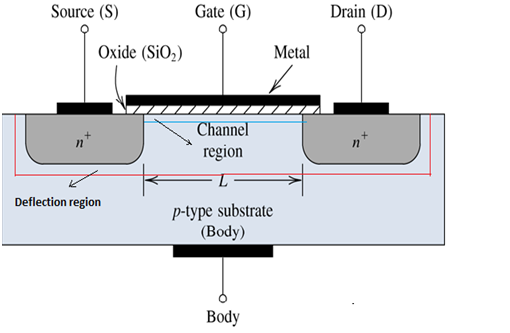
\includegraphics[width=0.5\linewidth]{figures/MOSFET-BLOCK-DIAGRAM.png}
  \caption{MOSFET Block diagram}
  \label{fig:}
\end{figure}

\subsection{N-type Enhancement-mode MOSFET}

\begin{figure}[H]
  \centering
  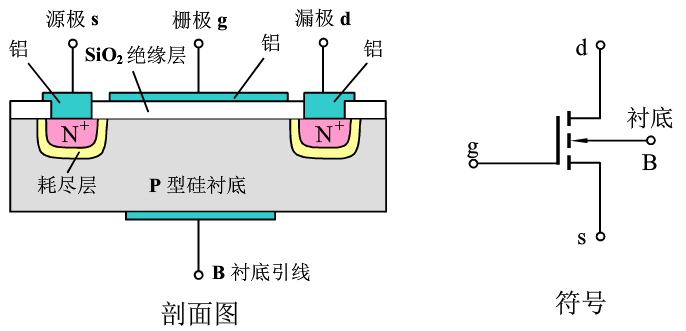
\includegraphics[width=0.7\linewidth]{figures/ENMOS}
  \label{fig:}
\end{figure}

Only when $V_{GS} > V_{TN} > 0$, N-Channel will be formed, MOSFET is conductive. $V_{TN}$ is called the Threshold Voltage.

\begin{figure}[H]
  \centering
  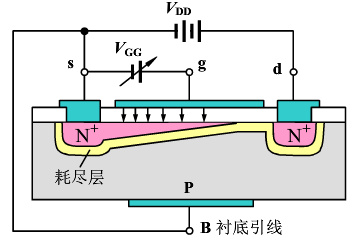
\includegraphics[width=0.5\linewidth]{figures/ENMOS2}
  \label{fig:}
\end{figure}

\begin{figure}[H]
  \centering
  \begin{subfigure}{.5\textwidth}
    \centering
    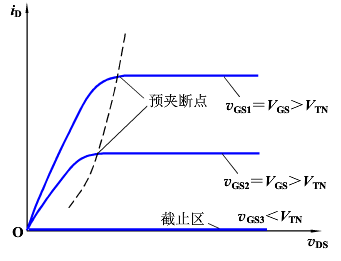
\includegraphics[width=\linewidth]{figures/ENMOSIV1}
    \label{fig:}
  \end{subfigure}%
  \begin{subfigure}{.5\textwidth}
    \centering
    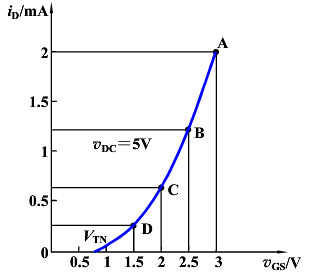
\includegraphics[width=\linewidth]{figures/ENMOSIV2}
    \label{fig:}
  \end{subfigure}
  \caption{The I-V Characteristic of N-type Enhancement-mode MOSFET}
  \label{fig:}
\end{figure}

\subsection{N-type Depletion-mode MOSFET}

The only difference between Enhancement-mode and Depletion-mode is the charges in oxide, which made $V_{TN} < 0$

\begin{figure}[H]
  \centering
  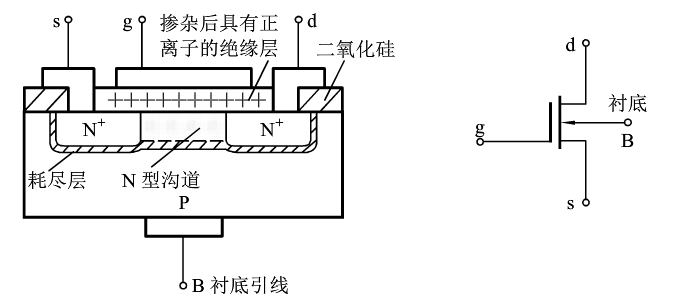
\includegraphics[width=0.7\linewidth]{figures/DNMOS}
  \label{fig:}
\end{figure}

\begin{figure}[H]
  \centering
  \begin{subfigure}{.5\textwidth}
    \centering
    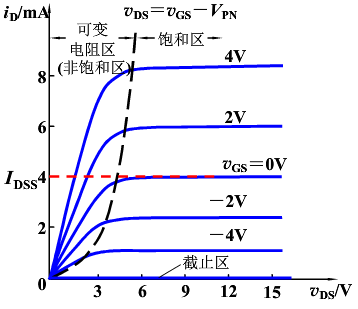
\includegraphics[width=\linewidth]{figures/DNMOSIV1}
    \label{fig:}
  \end{subfigure}%
  \begin{subfigure}{.5\textwidth}
    \centering
    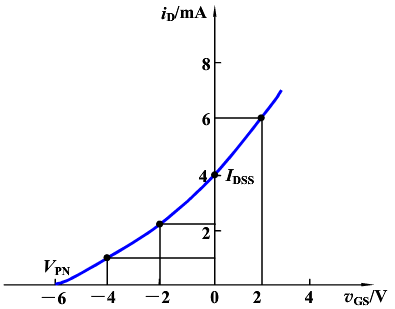
\includegraphics[width=\linewidth]{figures/DNMOSIV2}
    \label{fig:}
  \end{subfigure}
  \caption{The I-V Characteristic of N-type Depletion-mode MOSFET}
  \label{fig:}
\end{figure}

\subsection{P-type MOSFET}

\begin{figure}[H]
  \centering
  \begin{subfigure}{.3\textwidth}
    \centering
    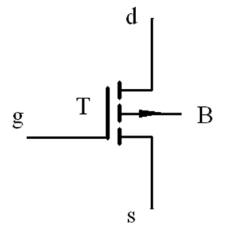
\includegraphics[width=\linewidth]{figures/EPMOS}
    \caption{Enhancement-mode}
    \label{fig:}
  \end{subfigure}%
  \begin{subfigure}{.3\textwidth}
    \centering
    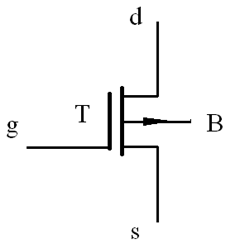
\includegraphics[width=\linewidth]{figures/DPMOS}
    \caption{Depletion-mode}
    \label{fig:}
  \end{subfigure}
  \caption{The Electronic Symbol of P-type MOSFET}
  \label{fig:}
\end{figure}

\begin{figure}[H]
  \centering
  \begin{subfigure}{.3\textwidth}
    \centering
    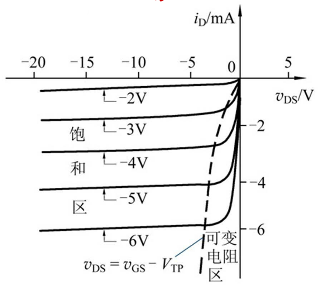
\includegraphics[width=\linewidth]{figures/PMOSIV1}
    \label{fig:}
  \end{subfigure}%
  \begin{subfigure}{.3\textwidth}
    \centering
    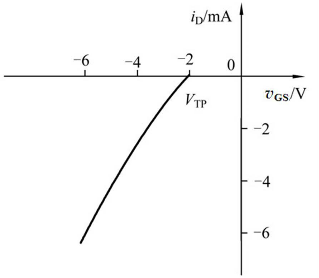
\includegraphics[width=\linewidth]{figures/PMOSIV2}
    \label{fig:}
  \end{subfigure}
  \caption{The I-V Characteristic of N-type Depletion-mode MOSFET}
  \label{fig:}
\end{figure}





%%% Local Variables:
%%% mode: latex
%%% TeX-master: "main"
%%% End:
